\chapter{直线}

在第一章，我们学习了曲线和方程两个重要概念，并学习了由曲线求它的方程的一般步骤. 现在，我们来研究最简单的曲线——直线. 先把它代数化（求出它的方程），然后利用它的方程来研究与它有关的一系列问题.这一章是坐标法的具体应用，是用代数方法研究几何问题的初步体现.


\section{直线的倾斜角和斜率}
过一个点并给出直线的方向能确定一条直线. 在坐标平面上，点可以用它的坐标表示，直线的方向如何表示呢？为此引入倾斜角的概念.

在坐标平面上，对于直线$\ell$，我们规定直线$\ell$的向上方向与$x$轴的正向所成的最小正角称为直线$\ell$的\textbf{倾斜角}（图2.1），记为$\alpha$．当直线$\ell$和$x$轴平行或重合时，规定它的倾斜角为$0^{\circ}$．由此，倾斜角的取值范围是$0^{\circ}\le \alpha<180^{\circ}$.

\begin{figure}[htp]
    \centering
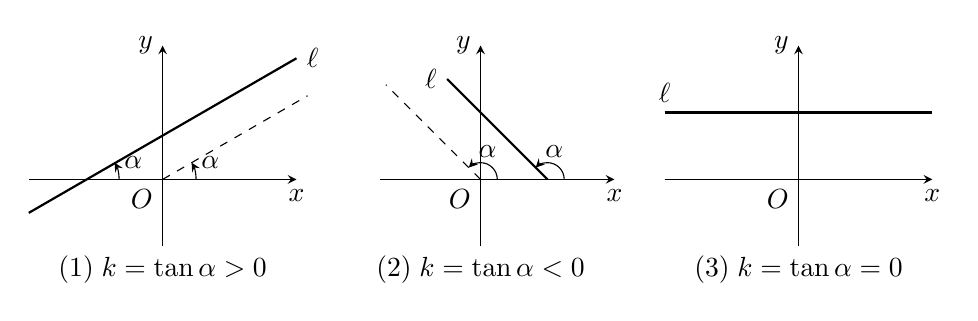
\begin{tikzpicture}[>=stealth, scale=.85]
\begin{scope}
\draw[->](-2,0)--(2,0)node[below]{$x$};
\draw[->](0,-1)node[below]{$(1)\; k=\tan\alpha>0$}--(0,2)node[left]{$y$};
\draw[thick](-2,-.5)--(2,1.81)node[right]{$\ell$};
\draw[dashed](0,0)--(30:2.5);
\draw[->](.5,0) arc (0:30:.5)node[right]{$\alpha$};
\draw[->](-.65,0) arc (0:30:.5)node[right]{$\alpha$};

\node[below left]{$O$};


\end{scope}    
\begin{scope}[xshift=4.75cm]
    \draw[->](-1.5,0)--(2,0)node[below]{$x$};
\draw[->](0,-1)node[below]{$(2)\; k=\tan\alpha<0$}--(0,2)node[left]{$y$};
\draw[thick](1,0)--(-.5,1.5)node[left]{$\ell$};
\draw[dashed](0,0)--(135:2);
\draw[->](.25,0) arc (0:135:.25)node[above right]{$\alpha$};
\draw[->](1.25,0) arc (0:135:.25)node[above right]{$\alpha$};

\node[below left]{$O$};

\end{scope}   
\begin{scope}[xshift=9.5cm]
    \draw[->](-2,0)--(2,0)node[below]{$x$};
\draw[->](0,-1)node[below]{$(3)\; k=\tan\alpha=0$}--(0,2)node[left]{$y$};
\draw[thick](-2,1)node[above]{$\ell$}--(2,1);
\node[below left]{$O$};

\end{scope}   
\end{tikzpicture}
    \caption{}
\end{figure}

因为一条直线只有一个方向，所以当平面直角坐标系选定以后，每一条直线能且只能与一个倾斜角相对应，反之亦
然. 因此，给出了倾斜角就给出了直线的方向.

倾斜角$\alpha$是一个几何对象. 为了用代数方法研究直线，我们再引进倾斜角的代数形式——斜率.

当$\alpha \ne 90^{\circ}$日时，$\alpha$ 的正切值称为直线$\ell$的斜率，记为$k$；

当$\alpha =90^{\circ}$时，也就是$\ell$垂直于$x$轴时，直线$\ell$没有斜率，即
\begin{equation}
\begin{split}
   k= \tan\alpha &\qquad (\alpha\ne 90^{\circ})\\
   k\text{不存在}&\qquad (\alpha= 90^{\circ})
\end{split} \tag{1}
\end{equation}

直线的斜率刻画了直线对于$x$轴的倾斜程度，它是描述直线方向的主要概念，因而将对直线的研究起重要的作用.

\begin{thm}
{思考题}
“在坐标平面上，每一条直线能且只能与一个斜率相对应，反之亦然”. 这句话是不正确的，应如何改正？    
\end{thm}

在坐标平面上，如果已知两个点$P_1(x_1,y_1)$、$P_2(x_2,y_2)$，那么过$P_1$、$P_2$的直线$\ell$就是确定的. 现在研究怎样用这两个点的坐标来表示$\ell$的斜率$k$. 由于$k$是$\alpha$ 的函数，$\alpha$被点$P_1$、$P_2$的位置决定，因此应从具体分析$P_1$、$P_2$的各种相对位置入手解决这个问题（图2.2）.

\begin{figure}[htp]
    \centering
\begin{tikzpicture}[>=stealth]
\begin{scope}
    \draw[->](-1,0)--(3,0)node[below]{$x$};
    \draw[->](0,-1)node[below]{$(1)$}--(0,2)node[left]{$y$};
\node[below left]{$O$};
\draw[thick](-1,1)--node[below]{$\ell_1$}(3,1);
\tkzDefPoints{.5/1/P_1, 2/1/P_2}
\tkzDrawPoints(P_1,P_2)
\tkzLabelPoints[above](P_1,P_2)
  \end{scope}
\begin{scope} [xshift=6.5cm, yshift=-.5cm]
    \draw[->](-1.5,0)--(2.5,0)node[below]{$x$};
    \draw[->](0,-.5)node[below]{$(2)$}--(0,2.5)node[left]{$y$};
\node[below left]{$O$};
\draw[domain=-1.25:1.75, thick, smooth]plot(\x,\x+.8)node[right]{$\ell_2$};
\draw[->](-.8+.35,0) arc (0:45:.35)node[right]{$\alpha$};
\tkzDefPoints{0.2/1/P_1, 1.5/2.3/P_2, 1.5/1/Q}
\tkzDrawPoints(P_1,P_2,Q)
\tkzLabelPoints[above left](P_2)
\tkzLabelPoints[above](P_1)
\tkzLabelPoints[above right](Q)
\draw[dashed](1.5,0)node[below]{$M_2$}--(1.5,2.3);
\draw[dashed](.2,1)--(1.75,1);
\end{scope}
\begin{scope}[yshift=-5cm]
    \draw[->](-1,0)--(2.5,0)node[below]{$x$};
    \draw[->](0,-1)node[below]{$(3)$}--(0,3)node[left]{$y$};
\node[below left]{$O$};
\draw[thick](1,0)--node[right]{$\ell_3$}(1,2.5);
\tkzDefPoints{1/.5/P_2, 1/1.75/P_1}
\tkzDrawPoints(P_1,P_2)
\tkzLabelPoints[right](P_1,P_2)
\end{scope}
\begin{scope}[xshift=6.5cm, yshift=-5cm]
    \draw[->](-1,0)--(3.5,0)node[below]{$x$};
    \draw[->](0,-1)node[below]{$(4)$}--(0,3)node[left]{$y$};
\node[below left]{$O$};
\draw[domain=-.5:2.5, thick]plot(\x, -\x+2)node[below]{$\ell_4$};
\draw[->](2+.25,0) arc (0:135:.25)node[above right]{$\alpha$};
\tkzDefPoints{.5/1.5/P_1, 1.5/.5/P_2, .5/.5/Q}
\tkzDrawPoints(P_1,P_2,Q)
\tkzLabelPoints[above right](P_1,P_2)
\tkzLabelPoints[below right](Q)
\draw[dashed](.5,0)node[below]{$M_1$}--(.5,1.5);
\draw[dashed](0,.5)--(1.5,.5);
\end{scope}
\end{tikzpicture}
    \caption{}
\end{figure}

对于$\ell_1:$ $\because\quad y_1= y_2,\; \ell_1\parallel x$轴，\qquad $\therefore \quad k=0$

对于$\ell_2:$ 过$P_1$作$P_1Q\bot y$轴，过$P_2$作$P_2M_2\bot x$轴，交
$P_{1}Q$ 于$Q$, 则$Q$ 的坐标是($x_2,y_1)$, 且$\alpha=\angle QP_1P_2$,
$$\tan \alpha=\frac{|QP_{2}|}{|P_{1}Q|}=\frac{y_{2}-y_{1}}{x_{2}-x_{1}}$$
若$P_1$, $P_2$的位置互换，则有
$$\tan \alpha=\frac{|QP_{1}|}{|P_{2}Q|}=\frac{y_{1}-y_{2}}{x_{1}-x_{2}}=\frac{y_{2}-y_{1}}{x_{2}-x_{1}}$$

对于$\ell_3:\; x_1=x_2$, $\ell_3\bot x$ 轴，$k$ 不存在；


对于$\ell_4:$ 过$P_1$作$P_1M_1\bot x$轴，作$P_2Q\bot y$ 轴 交 $P_1M_1$于
$Q$,
则 
\[\begin{split}
    \tan\alpha &=\tan(180^{\circ}-\angle QP_{2}P_{1})=-\tan \angle QP_{2}P_{1}\\
    &=-\frac{|P_{1}Q|}{|QP_{2}|}=-\frac{y_{1}-y_{2}}{x_{2}-x_{1}}=\frac{y_{2}-y_{1}}{x_{2}-x_{1}}
\end{split}\]
若$P_1$, $P_2$的位置互换，则有
$$\tan \alpha=-\frac{|P_{2}Q|}{|QP_{1}|}=-\frac{y_{2}-y_{1}}{x_{1}-x_{2}}=\frac{y_{2}-y_{1}}{x_{2}-x_{1}}$$

回 过 头 来 , 对 于 $\ell_{1}$, $k= 0$, 因为 $y_1=y_2$, $x_1\neq x_2$, 所以也
可以写成 $k=\frac{y_2-y_1}{x_2-x_1}$的形式。这样，我们就得到了
\begin{equation}
    \begin{split}
    k=\frac{y_2-y_1}{x_2-x_1} &\qquad \text{当}x_1\ne x_2\\
    k\text{不存在} &\qquad \text{当}x_1= x_2
    \end{split}\tag{2}
\end{equation}
公式(2)直接用$\ell$上两个点的坐标表示出了直线的斜率. 从而为用坐标法研究直线提供了方便.

\begin{thm}
  {思考题}
若直线$\ell$不与$x$轴垂直，并且$\ell$上有三个点：$P_1(x_1,y_1)$、$P_2(x_2,y_2)$、$P_3(x_3,y_3)$. 用$P_1$、$P_2$的坐标算出的$k$值与用$P_1$、$P_3$或$P_2$、$P_3$的坐标算出的$k'$值相同吗？为什么？  
\end{thm}

\begin{example}
    如图2.3，直线$\ell_1$的倾斜角$\alpha_1=30^{\circ}$，直线$\ell_2\bot\ell_1$，求$\ell_1$、$\ell_2$的斜率.
\end{example}

\begin{solution}
$\ell_1$的斜率 $k_1=\tan\alpha_1=\tan30^{\circ}=\frac{\sqrt{3}}{3}$

$\because\quad \ell_2\bot\ell_1$，

$\therefore\quad \ell_2$的倾斜角 $\alpha_2=\alpha_1+90^{\circ}=30^{\circ}+90^{\circ}=120^{\circ}$

$\ell_2$的斜率 $k_2=\tan\alpha_2=\tan120^{\circ}=-\tan 60^{\circ}=-\sqrt{3}$
\end{solution}

\noindent
\begin{minipage}{.45\textwidth}
    \centering
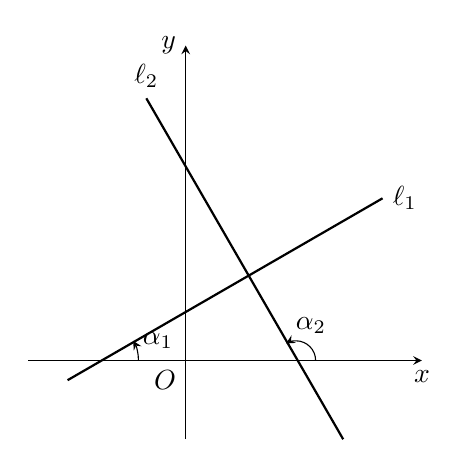
\begin{tikzpicture}[>=stealth]
    \draw[->](-2,0)--(3,0)node[below]{$x$};
    \draw[->](0,-1)--(0,4)node[left]{$y$};
\node[below left]{$O$};

\draw[thick](-1.5,-.25)--(2.5, 1.81+.25)node[right]{$\ell_1$};
\draw[->](-.6,0) arc (0:30:.5)node[right]{$\alpha_1$};
\draw[thick](2,-1)--(-.5, 2.5*1.732-1)node[above]{$\ell_2$};
\draw[->](1.9-.25,0) arc (0:120:.25)node[above right]{$\alpha_2$};

\end{tikzpicture}
\captionof{figure}{}
\end{minipage}
\hfill
\begin{minipage}{.45\textwidth}
    \centering
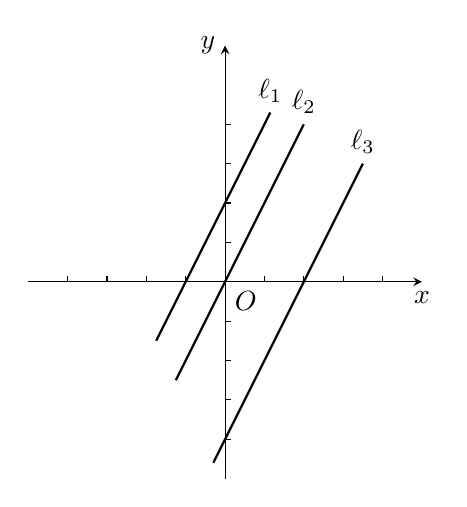
\begin{tikzpicture}[>=stealth, scale=.5]
    \draw[->](-5,0)--(5,0)node[below]{$x$};
    \draw[->](0,-5)--(0,6)node[left]{$y$};
\node[below right]{$O$};
\draw[domain=-1.75:1.15, thick]plot(\x, 2*\x+2)node[above]{$\ell_1$};
\draw[domain=-1.25:2, thick]plot(\x, 2*\x)node[above]{$\ell_2$};
\draw[domain=-.3:3.5, thick]plot(\x, 2*\x-4)node[above]{$\ell_3$};
\foreach \x in {-4,-3,...,4}
{
    \draw(\x,0)--(\x,.15);
    \draw(0,\x)--(.15,\x);
}
\end{tikzpicture} 
\captionof{figure}{}
\end{minipage}

\begin{example}
    求经过$A(-2,0)$、$B(-5,3)$两点的直线的斜率与倾斜角．
\end{example}

\begin{solution}
    由公式(2)，得
\[k=\frac{y_2-y_1}{x_2-x_1}=\frac{3-0}{-5-(-2)}=-1\]
再由公式(1)，得 $-1=\tan\alpha$.

$\because\quad 0\le \alpha<180^{\circ},\qquad \therefore\quad \alpha =135^{\circ}$.

$\therefore\quad$这条直线的斜率是$-1$，倾斜角是$135^{\circ}$．
\end{solution}

最后，再引进直线的纵截距和横截距的概念.

在坐标平面上，对于不平行于$y$轴的直线$\ell$，它与$y$轴交点的纵坐标称为它的\textbf{纵截距}.

如图2.4中的直线$\ell_1$、$\ell_2$、$\ell_3$的纵截距分别是2、0、$-4$．若$\ell\parallel y$轴，它的纵截距没有意义（图2.2(3)）．

同时，对于不平行$x$轴的直线$\ell$，它与$x$轴交点的横坐标称为它的\textbf{横截距}.
如图2.4中的直线$\ell_1$、$\ell_2$、$\ell_3$的横截距分别是$-1$、0、2．若$\ell\parallel x$轴，它的横截距也没有意义［图2.2(1)］．

直线的斜率和截距是在坐标系中刻画直线位置的两个重要参数，应结合图形掌握它们的几何意义.

\begin{thm}
    {思考题} 斜率和截距具有什么特点时直线一定通过II、III、IV象限？I、IV、III象限？
\end{thm}

\begin{ex}
\begin{enumerate}
    \item 填空
\begin{enumerate}[(1)]
    \item 斜率$k$的取值范围是\blank
    \item 当$k>0$时，直线$\ell$一定通过\blank 象限;
    \item 当$k<0$时，直线$\ell$一定通过\blank 象限；
    \item 当$k=0$时，直线$\ell$或通过\blank 象限，或通过\blank 象限，或者\blank; \blank;
    \item 当$k$不存在时，直线$\ell$或通过\blank，或\blank, 或者\blank.
\end{enumerate}

    \item 已知直线的倾角为$\alpha$，求它的斜率
\begin{multicols}{2}
\begin{enumerate}[(1)]
\item $\alpha =0^{\circ}$;
\item $0^{\circ}<\alpha <90^{\circ}$;
\item $\alpha =90^{\circ}$;
\item $90^{\circ}<\alpha <180^{\circ}$.
\end{enumerate}    
\end{multicols}
    \item 求经过下列两点的直线的斜率和倾斜角：
\begin{multicols}{2}
\begin{enumerate}[(1)]
\item $C(-1,\sqrt{3})$ 与 $D(0,0)$
\item $A(3,-8)$ 与 $B(-2,6)$
\item $E(\sqrt{3},-\sqrt{2})$ 与 $F(-\sqrt{2},\sqrt{3})$
\item $G(-2,5)$ 与 $H(-2,-3)$  
\end{enumerate}    
\end{multicols}
\end{enumerate}
\end{ex}

\section{直线方程的几种形式}
确定一条直线需要两个条件，本节将就坐标平面上两个条件的不同给法，根据1.5节的理论分别求出直线$\ell$的不同形式的方程.

\begin{thm}{情况1}
已知直线$\ell$过点$P_0(x_0,y_0)$且斜率是$k$，求直线$\ell$的方程.
\end{thm}

\noindent
\begin{minipage}{.55\textwidth}
\CTEXindent
如图2.5，设$\ell$上异于$P_0$的动点为$P(x,y)$，点$P$运动的规律是过$P_0$、$P$的直线的斜率始终是$k$，即
\[\frac{y-y_0}{x-x_0}=k\quad (x\ne x_0)\]

化简，得
\begin{equation}
    y-y_0=k(x-x_0) \tag{1}
\end{equation}
\end{minipage}
\hfill
\begin{minipage}{.4\textwidth}
\centering
\begin{tikzpicture}[>=stealth]
\draw[->](-2,0)--(3,0)node[below]{$x$};
\draw[->](0,-1)--(0,2.5)node[left]{$y$};
\draw[thick](-1.5, -.2)--(2.5,1.8)node[above]{$\ell$};
\node[below left]{$O$};
\tkzDefPoints{.5/.8/P_0, 2/1.55/P}
\tkzDrawPoints(P_0,P)
\node at (P_0)[below right]{$P_0(x_0,y_0)$};
\node at (P)[below right]{$P(x,y)$};

\end{tikzpicture}
\captionof{figure}{}
\end{minipage}

\begin{proof}
由(1)式的推导，知道，凡是$\ell$上的点其坐标都满足方程(1). 以下证明：(1)的任一个解对应的点都在$\ell$上.

设$\begin{cases}
    x=x_1\\y=y_1
\end{cases}$
是(1)的任一解，即
\begin{equation}
    y_1-y_0=k(x_1-x_0)\tag{$1'$}
\end{equation}

分两种可能：
\begin{enumerate}[(i)]
\item 当$x_1=x_0$时，由($1'$)知$y_1=y_0$，由此，$P_1(x_1,y_1)$与$P_0(x_0,y_0)$重合，

$\therefore\quad P_1(x_1,y_1)$在$\ell$上；
\item 当$x_1\ne x_0$时，由($1'$)得，
\[\frac{y_1-y_0}{x_1-x_0}=k\]
这说明过$P_0$、$P_1$的直线的斜率也是$k$，

$\therefore\quad P_1(x_1,y_1)$在$\ell$上.
\end{enumerate}
\end{proof}

根据曲线与方程的定义. 直线$\ell$的方程是(1).

方程(1)是由直线$\ell$上的一个点和$\ell$的斜率确定的，称为直线方程的\textbf{点斜式}.

当直线$\ell$过点$P_0(x_0,y_0)$，且垂直$y$轴时（图2.6），倾斜角$\alpha=0$, $k=\tan\alpha=0$，由(1)得$\ell$的方程为
\[y-y_0=0(x-x_0)\]
即
\begin{equation}
    y=y_0 \tag{2}
\end{equation}

\noindent
\begin{minipage}{.45\textwidth}
\centering
\begin{tikzpicture}[>=stealth]
    \draw[->](-1,0)--(3.5,0)node[below]{$x$};
\draw[->](0,-1)--(0,3)node[left]{$y$};
\node[below left]{$O$};
\draw[thick](-1,2)--(3,2);
\draw[fill](1.5,2)node[below]{$P_0(x_0,y_0)$} circle(1.5pt);
\tkzDefPoints{0/3/A, 0/2/B, 1/2/C}
\tkzMarkRightAngle(A,B,C)
\end{tikzpicture}
\captionof{figure}{}
\end{minipage}\hfill
\begin{minipage}{.45\textwidth}
    \centering
\begin{tikzpicture}[>=stealth]
    \draw[->](-1,0)--(3.5,0)node[below]{$x$};
    \draw[->](0,-1)--(0,3)node[left]{$y$};
\node[below left]{$O$};

\draw[thick](1.5,-1)--(1.5,2.5);
\draw[fill](1.5,2)node[right]{$P_0(x_0,y_0)$} circle(1.5pt);
\tkzDefPoints{1.5/3/A, 1.5/0/B, 2/0/C}
\tkzMarkRightAngle(A,B,C)

\end{tikzpicture}
\captionof{figure}{}

\end{minipage}

当直线$\ell$过$P_0(x_0,y_0)$，且垂直于$x$轴时（图2.7），倾斜角$\alpha=\frac{\pi}{2}$，$k$不存在，$\ell$的方程不能用(1)表示. 但$\ell$上任一点的横坐标都是，这时，直线的方程是：
\begin{equation}
    x=x_0 \tag{3}
\end{equation}


\begin{thm}
  {情况2} 已知直线$\ell$的斜率是$k$，纵截距是$b$，求$\ell$的方程.  
\end{thm}

此时$\ell$过$(0,b)$点，且斜率为$k$．由公式(1)得
\[y-b=k(x-0)\]
即
\begin{equation}
    y=kx+b \tag{4}
\end{equation}

方程(4)称为直线方程的\textbf{斜截式}.

\begin{thm}
  {情况3} 已知直线$\ell$通过两点$P_1(x_1,y_1)$、$P_2(x_2,y_2)$，求$\ell$的方程.  
\end{thm}

应考虑横坐标$x_1$与$x_2$的关系：
\begin{enumerate}[(1)]
\item 当$x_1=x_2$时，$\ell\bot x$轴，$\ell$的方程是
\[x=x_1\]
\item 当$x_1\ne x_2$时，可转化成点斜式处理. 此时$\ell$的斜率，所以$\ell$的方程可写成
\begin{equation}
y-y_1=\frac{y_2-y_1}{x_2-x_1}(x-x_1)\quad (x_1\ne x_2) \tag{5}    
\end{equation}

方程(5)称为直线方程的\textbf{两点式}.
\end{enumerate}

当$y_2\ne y_1$时，方程(5)还可以写成
\begin{equation}
    \frac{y-y_1}{y_2-y_1}=\frac{x-x_1}{x_2-x_1}\qquad (x_1\ne x_2,\; y_1\ne y_2) \tag{5}
\end{equation}

\begin{thm}
    {情况4} 已知直线$\ell$的纵截距、横截距分别是$b$、$a$（其中$a\ne 0$, $b\ne 0$），求$\ell$的方程（图2.8）．
\end{thm}

\noindent
\begin{minipage}{.55\textwidth}
    \CTEXindent
这种情况可转化成两点式解决. 事实上$\ell$过$P_1(a,0)$、$P_2(0,b)$，代入(5)，得
\[y-0=\frac{b-0}{0-a}(x-a)\]
化简，得
\begin{equation}
    \frac{x}{a}+\frac{y}{b}=1  \tag{6}
\end{equation}    
\end{minipage}
\hfill
\begin{minipage}{.4\textwidth}
\centering
\begin{tikzpicture}[>=stealth]
    \draw[->](-2,0)--(2.5,0)node[below]{$x$};
    \draw[->](0,-1)--(0,2.5)node[left]{$y$};
\node[below left]{$O$};
\tkzDefPoints{-1.5/0/A, 0/1/B}
\tkzDrawLine[add = .2 and 1.3](A,B)
\node at (A)[below]{$a$};
\node at (B)[right]{$b$};
\end{tikzpicture}
\captionof{figure}{}
\end{minipage}


方程(6)称为直线方程的\textbf{截距式}.

到此为止，我们学过了四种形式的方程，它们都表示直线，它们是：
\begin{align}
y-y_0&=k(x-x_0)  \tag{1}\\
y&=kx+b \tag{2}\\
\frac{y-y_1}{y_2-y_1}&=\frac{x-x_1}{x_2-x_1}\quad (x_1\ne x_2,\; y_1\ne y_2)\tag{3}\\
\frac{x}{a}+\frac{y}{b}&=1\quad (a\ne0,\; b\ne 0)\tag{4}
\end{align}

应该知道，不是平面上的所有直线都能写成上述这些形式的方程. 平行于$y$轴的直线不能写成(1)(2)(3)(4)这四种形式，平行于$x$轴的直线不能写成(4)的形式.

上面得到了直线方程的四种特殊形式. 这些方程从代数上看都是关于$x$、$y$的一次方程. 这一事实启迪我们思考：
\begin{enumerate}[(i)]
\item $xOy$平面上的任一条直线，其方程是否都是关于$x$、$y$的一次方程？
\item 关于$x$、$y$的一次方程$Ax+By+C=0$是否都表示$xOy$平面上的一条直线？
\end{enumerate}


这两个问题是直线与一次方程的关系问题，现在分析如下：
\begin{enumerate}[(i)]
    \item $xOy$平面上的所有直线，根据倾斜角$\alpha$是否等于$90^{\circ}$，可以分作两类：

    当$\alpha\ne 90^{\circ}$时，直线的斜率记为$k$，其方程总可以写成$y=kx+b$，
它是关于的一次方程.

当$\alpha=90^{\circ}$时，其方程总可以写成$x=x_0$，即
\[x+0y-x_0=0\]
这个方程仍可以看做关于$x$、$y$的一次方程.

所以，$xOy$平面上的任一直线，其方程都是关于$x$、$y$的一次方程.
\item 要回答关于$x$、$y$的一次方程$Ax+By+C=0$是否都表示直线，讨论如下：

当$B\ne 0$时，方程$Ax+By+C=0$可化成
\[y=-\frac{A}{B}x-\frac{C}{B}\]
这就是直线的斜截式方程，其中$k=-\frac{A}{B}$, $b=-\frac{C}{B}$；

当$B=0$时，则有$A\ne 0$，$Ax+By+C=0$可以写成
\[x=-\frac{C}{A}\]
它表示与$y$轴平行的直线.

所以，关于$x$、$y$的任一个一次方程$Ax+By+C=0$都表示一条直线.
\end{enumerate}

这样，就得到了
\begin{thm}
{定理}
\begin{enumerate}[(i)]
\item $xOy$平面上的任意一条直线，其方程都是关于$x$、$y$的一次方程；
\item 任意一个关于$x$、$y$的一次方程$Ax+By+C=0$（$A$、$B$不同时为零），都表示$xOy$平面上的一条直线.    
\end{enumerate} 
\end{thm}

这个定理很重要，它是上述直线方程的特殊形式在理论上的概括，它揭示了坐标平面上的直线与关于$x$、$y$的一次方程的联系，根据这种联系，研究直线的几何问题就可以和研究一次方程的代数问题互化了.

我们把方程
\begin{equation}
    Ax+By+C=0 \tag{7}
\end{equation}
（其中$A$、$B$不全为零）叫做直线方程的\textbf{一般式}.

对各种形式的直线方程，应注意每个方程适用的条件，并能根据需要灵活地选择直线方程的某种形式进行解题.

\begin{example}
直线$\ell$的方程是$\sqrt{3}x+3y+6=0$\hfill (1)

求$\ell$的斜率、倾斜角和纵截距。
\end{example}

\begin{analyze}
    欲求$k$和纵截距$b$, 须把(1)变成斜截式.
\end{analyze}

\begin{solution}
    由(1)得
\begin{equation}
    y=-\frac{\sqrt{3}}3x-2 \tag{2}
\end{equation}

$\therefore\quad k= - \frac {\sqrt {3}}3$，倾斜角$\alpha=\pi-\arctan\frac{\sqrt{3}}{3}=\frac{5}{6}\pi$, 
纵截距$b=-2$.
\end{solution}

\begin{example}
    直线$\ell$的方程是$\sqrt3x+3y+6=0$\hfill (1)

求$\ell$的横截距和纵截距。
\end{example}

\begin{analyze}
    欲求双截距$a$ 和$b$, 可以采用两种方法：
\end{analyze}

\begin{solution}
\textbf{解法1：}把(1)变成截距式
\[\begin{split}
    \sqrt{3}x+3y&=-6\\
    \frac{\sqrt{3}}{-6}x+\frac{3}{-6}y&=1\\
\frac{x}{-2\sqrt{3}}+\frac{y}{-2}&=1
\end{split}\]
$\therefore\quad a= - 2\sqrt {3},\quad b=-2$.    

\textbf{解法 2：} 用求交点的方法来解。

在(1)中令$y=0$, 得$\sqrt{3} x=-6,\quad  x=-2 \sqrt{3}$,

$\therefore a= - 2\sqrt {3}$ ;    

在(1)中令$x=0$, 得$3y=-6,\quad  y=-2 \sqrt{3}$,

$\therefore b= - 2$.    
\end{solution}

\begin{example}
直线$\ell$的横截距是$-3$，斜率是$-2$，求$\ell$的一般式．
\end{example}

\begin{analyze}
    因为已知斜率和横截距，所以，可写出点斜式方程，再化成一般式.
\end{analyze}

\begin{solution}
$\because\quad \ell$过$(-3,0)$，$k=-2$

$\therefore\quad\ell$的方程是$y=-2(x+3)$. 
即$2x+y+6=0$.
\end{solution}

\begin{thm}
    {思考题} 从一般式入手，能解此题吗？试试看.
\end{thm}

\begin{ex}
\begin{enumerate}
    \item 填空：
\begin{enumerate}[(1)]
\item 经过点$(-2,-3)$，且斜率为$-1$的直线方程是\blank ;
\item 经过点$(-1,-5)$，且倾斜角为$\frac{5\pi}{6}$的直线方程是\blank ;
\item 经过点$(-1,-4)$，且垂直$y$轴的直线方程是\blank ;
\item 经过点$(2,-3)$，且垂直$x$轴的直线方程是\blank ;
\item 斜率为$-2$，纵截距为$-4$的直线方程是\blank；
\item 倾斜角为$\frac{\pi}{3}$，纵截距为$-2$的直线方程是\blank .
\end{enumerate}

    \item 直线$\ell$的方程是$ax+by+c=0$，当系数$a$、$b$、$c$满足什么条件时：
\begin{enumerate}[(1)]
\begin{multicols}{2}
    \item $\ell\bot x$轴;
    \item $\ell$与$x$轴重合；
    \item $\ell$过原点；
    \item $\ell$与两轴都相交；
    \item $\ell$与$x$正半轴相交；    
\end{multicols}
    \item $\ell$的倾斜角为$\frac{\pi}{3}$，且纵截距为2；
    \item $\ell$与坐标轴围成等腰三角形．
\end{enumerate}
\end{enumerate}
\end{ex}

\section*{习题一}
\begin{center}
    \bfseries A
\end{center}

\begin{enumerate}
    \item 若$a$、$b$、$c$是两两不等的实数，求经过下列两点的直线的倾斜角：
\begin{multicols}{2}
\begin{enumerate}[(1)]
\item $A(a,c)$与$B(b,c)$
\item $C(a,b)$与$D(a,c)$
\item $P(b,b+c)$与$Q(a,c+a)$
\end{enumerate}
\end{multicols}

    \item 直线$\ell$的方程是$2x+y-2\sqrt{6}=0$，求其横截距和纵截距.
    \item 已知直线$\ell$的方程是$x-2y+6=0$. 求$\ell$的斜率、倾斜角、横纵截距，并画图.
\end{enumerate}

\begin{center}
    \bfseries B
\end{center}

\begin{enumerate}\setcounter{enumi}{3}
    \item 已知三点$A$、$B$、$C$，若直线$AB$、$AC$的斜率相同，证明这\textbf{三点共线}.
\item     证明：由方程
    \[ax+by+c=0, \quad ax-by+c=0,\quad b\ne 0\]
    确定的两条直线关于$x$轴对称.
\item 证明：直线$ax+by+c=0,\quad (a,b,c\ne 0)$
    和坐标轴围成的三角形的面积为$S=\frac{c^2}{2|ab|}$.
\end{enumerate}

\section{两条直线所成的角}

\noindent
\begin{minipage}{.55\textwidth}
\CTEXindent 
两条直线相交构成四个角，它们是两对对顶角. 为了区别它们，先引入$\ell_1$到$\ell_2$的角的概念．图2.9中的$\theta_{1-2}$表示$\ell_1$绕交点，逆时针第一次转到$\ell_2$形成的角，称为$\ell_1$到$\ell_2$的角；$\theta_{2-1}$表示$\ell_2$绕交点逆时针第一次转到$\ell_1$形成的角，称为$\ell_2$到$\ell_1$的角．

根据上述定义，不难得出：
\end{minipage}
\hfill
\begin{minipage}{.35\textwidth}
\centering
\begin{tikzpicture}[>=stealth, scale=1.3]
\tkzDefPoint(150:1.5){A}
\tkzDefPoint(-30:1.5){B}
\tkzDefPoint(35:1.5){A'}
\tkzDefPoint(35-180:1.5){B'}
\tkzDefPoint(0,0){O}
\draw[thick](A)--(B)node[below]{$\ell_2$};
\draw[thick](B')--(A')node[above]{$\ell_1$};
\tkzMarkAngles[mark=none, ->, size=.4cm](A',O,A)
\tkzMarkAngles[mark=none, ->, size=.3cm](B,O,A')
\tkzLabelAngle[pos=.8](B,O,A'){$\theta_{2-1}$}
\tkzLabelAngle[pos=.7](A',O,A){$\theta_{1-2}$}


\end{tikzpicture}
\captionof{figure}{}
\end{minipage}


\[0<\theta_{1-2}<\pi,\quad 0<\theta_{2-1}<\pi,\quad \theta_{1-2}+\theta_{2-1}=\pi\]

在坐标平面上，$\theta_{1-2}$或$\theta_{2-1}$能否用两条直线的倾斜角表示呢？

先看特殊情况：当至少有一条直线垂直于坐标轴时（图2.10），到角极易算出，请读者试试看．

\begin{figure}[htp]
    \centering
\begin{tikzpicture}[>=stealth]
\begin{scope}
        \draw[->](-2,0)--(3,0)node[below]{$x$};
        \draw[->](0,-1)--(0,4)node[left]{$y$};
        \node[below left]{$O$};
    \draw(1.5,-.75)--(1.5,3.5)node[above]{$\ell_1$};
    
    \tkzDefPoints{0/1/A, 1.5/2.5/B}
    \tkzDrawLine[add=1 and .7](A,B)    
    \draw[->](-.5,0) arc (0:45:.5)node[right]{$\alpha_2$};
    \draw[->](1.5,2.25) arc (-90:45:.25)node[below right]{$\theta_{1-2}$};
    \draw[->](1.5+.4,2.5+.4) arc (45:90:.4*1.414)node[above right]{$\theta_{2-1}$};
    \node at (1.5+1.25,2.5+1.25){$\ell_2$};
    \node at (.5,-1){(1)};
\end{scope}
\begin{scope}[xshift=6cm]
    \draw[->](-1,0)--(4,0)node[below]{$x$};
    \draw[->](0,-1)--(0,4)node[left]{$y$};
    \node[below left]{$O$};
\draw(-1,2)--(3.5,2)node[right]{$\ell_1$};
\node at (1.5,-1){(2)};

\tkzDefPoints{1/2/A, 2/0/B}
\tkzDrawLine[add=.7 and .6](A,B)    
\draw[->](2.5,0) arc (0:116.6:.5)node[above right]{$\alpha_2$};
\draw[->](1.5,2) arc (0:116.6:.5)node[above right]{$\theta_{1-2}$};
\draw[<-](1.6,2) arc (0:-63.4:.6)node[right]{$\theta_{2-1}$};
\node at (0,3.65)[right]{$\ell_2$};
\end{scope}
\end{tikzpicture}
    \caption{}
\end{figure}



现在研究一般情况：已知图（2.11）
\begin{itemize}
    \item $\ell_1:\; y=k_1x+b_1$，倾斜角为$\alpha_1$;
    \item $\ell_2:\; y=k_2x+b_2$，倾斜角为$\alpha_2$.
\end{itemize}

\begin{figure}[htp]
    \centering
\begin{tikzpicture}[>=stealth]
\begin{scope}
    \draw[->](-2,0)--(3,0)node[below]{$x$};
    \draw[->](0,-1)--(0,3)node[left]{$y$};
    \node[below left]{$O$};
\tkzDefPoints{-1/0/A, 2/0/B, 1/2/C, 4/0/B'}
\tkzDrawLine[add=.3 and .4](A,C)  
\tkzDrawLine[add=.3 and .4](B,C)  
\node at (1,-1){(1)};
\tkzMarkAngles[mark=none, size=.5cm, ->](B,A,C B',B,C)
\tkzLabelAngle[pos=.8](B,A,C){$\alpha_1$}
\tkzLabelAngle[pos=.8](B',B,C){$\alpha_2$}
\node (D) at (.5,3){$\ell_2$};
\node (D') at (1.85,3){$\ell_1$};
\tkzMarkAngles[mark=none, size=.4cm, ->](D',C,D)
\tkzLabelAngle[pos=.6](D',C,D){$\theta_{1-2}$}

\end{scope}
\begin{scope}[xshift=6cm]
    \draw[->](-1,0)--(4,0)node[below]{$x$};
    \draw[->](0,-1)--(0,3)node[left]{$y$};
    \node[below left]{$O$};
    \tkzDefPoints{.5/0/A, 3/0/B, 2/1.5/C, 4/0/B'}
    \tkzDrawLine[add=.5 and .6](A,C)  
    \tkzDrawLine[add=.5 and .6](B,C)   
    \node at (1.5,-1){(2)};
    \tkzMarkAngles[mark=none, size=.5cm, ->](B,A,C B',B,C)
    \tkzMarkAngles[mark=none, size=.4cm, ->](C,B,A)
    \tkzLabelAngle[pos=.8](B,A,C){$\alpha_2$}
    \tkzLabelAngle[pos=.8](B',B,C){$\alpha_1$}
    \tkzLabelAngle[pos=.7](C,B,A){$\beta$}
    \node (D) at (3.1,2.65){$\ell_2$};
    \node (D') at (1.5,2.65){$\ell_1$};
    \tkzMarkAngles[mark=none, size=.4cm, ->](B,C,D)
    \tkzLabelAngle[pos=.8](B,C,D){$\theta_{1-2}$}

\end{scope}
\end{tikzpicture}
    \caption{}
\end{figure}


容易看出，$$\theta_{1-2}=\alpha_2-\alpha_1$$
或
\begin{equation}
    \theta_{1-2}=\alpha_2+\beta =\alpha_2+(\pi-\alpha_1)=\pi+(\alpha_2-\alpha_1)\tag{1}
\end{equation}

我们知道，直线的倾斜角和斜率有直接的关系.那么，这里得到的$\theta_{1-2}$能否用$\ell_1$、$\ell_2$的斜率$k_1$、$k_2$表示呢？为此，只要对(1)两边取正切即可：
\begin{equation}
\tan\theta_{1-2}=\frac{\tan\alpha_2-\tan\alpha_1}{1+\tan\alpha_2\tan\alpha_1}=\frac{k_2-k_1}{1+k_2k_1}\quad (1+k_1k_2\ne 0) \tag{2}
\end{equation}

公式(2)称为\textbf{到角公式}．对它应注意：
\begin{enumerate}[(i)]
    \item $\theta_{1-2}$的几何意义；
    \item 公式的结构特征；
    \item 当$\theta_{1-2}$, $\alpha_1$, $\alpha_2$都不等于$\frac{\pi}{2}$时才能使用这个公式.
\end{enumerate}

两个到角$\theta_{1-2}$与$\theta_{2-1}$中，较小的一个更加常用，称为两条直线\textbf{所成的角}（简称\textbf{夹角}）.显然夹角的取值范围是$\left(0,\frac{\pi}{2}\right]$. 若要求夹角$\theta$，由(2)可得
\begin{equation}
    \tan\theta =\left|\frac{k_2-k_1}{1+k_2k_+1}\right|
\end{equation}

\begin{example}
    求直线$\ell_1:\; 2x+y-2=0$和$\ell_2:\; 3x-y+2=0$的夹角.
\end{example}


\begin{solution}
    $\ell_1,\ell_2$的斜率分别是$k_1=-2$, $k_2=3$, 由夹角公式(3)得
\[\tan\theta=\left|\frac{3-(-2)}{1+3\cdot(-2)}\right|=1,\qquad \theta=45^{\circ}\]
$\therefore \quad \ell_1,\ell_2$的夹角为$45^{\circ}$.
\end{solution}


\begin{example}
    已知：$\ell_1:\; x-y-5=0$ 和$\ell_2:\; ax+y=0$, 且$\theta_{1-2}=75^{\circ}$, 求$a$.
\end{example}

\begin{solution}
    $\ell_1$、$\ell_2$的斜率是$k_1=1$, $k_2=-a$. $\theta_{1-2}=75^\circ$. 由公式
$\tan\theta_{1-2}=\frac{k_2-k_1}{1+k_2k_1}$，得
    $$\tan 75^{\circ}=\frac{-a-1}{1+1\cdot(-a)}$$

解这个关于$a$的方程（注意$\tan75^{\circ}=2+\sqrt{3}$）得$a=\sqrt{3}$.
\end{solution}


\begin{example}
 过点$P(2,-1)$引直线$\ell'$，使它与直线$\ell:\; 5x-2y+3=0$ 的夹角为$45^{\circ}$. 求 $\ell'$的方程.
\end{example}

\begin{solution}
    只要求出$\ell'$的斜率$k'$就行了. 因为$\ell$的斜率$k=\frac{5}{2}$, 由夹角公式，得
\begin{minipage}{.55\textwidth}
\[\tan45^{\circ}=\left|\frac{k'-k}{1+k'k}\right|=\left|\frac{k'-\frac{5}{2}}{1+\frac{5}{2}k'}\right|\]
即
\[\frac{k'-\frac{5}{2}}{1+\frac{5}{2}k'}=\pm 1 \quad  \Rightarrow \quad \frac{2k'-5}{2+5k'}=\pm 1\]
解得：$k'_1=-\frac{7}{3},\quad k'_2=\frac{3}{7}$. 从而，$\ell'$有两条（图2.12），它们的方程分别是
\[y+1=-\frac{7}{3}(x-2)\quad \text{和}\quad y+1=\frac{3}{7}(x-2)\]
\end{minipage}
\hfill
\begin{minipage}{.4\textwidth}
\centering
\begin{tikzpicture}[>=stealth, scale=.8]
\draw[->](-2.5,0)--(3.5,0)node[above]{$x$};
\draw[->](0,-4)--(0,4)node[left]{$y$};
\node[below left]{$O$};
\draw[domain=-2:.8, smooth, very thick]plot(\x, 2.5*\x+1.5)node[above]{$\ell$};
\tkzDefPoints{.45/2.62/A, -1.62/-2.55/B, 2/-1/P}
\tkzDrawPoints(A,B,P)
\tkzDrawLines[add = .2 and .4](A,P B,P)
\tkzMarkAngles[size=.5, mark=none](B,A,P P,B,A)
\tkzLabelAngle[pos=.85](B,A,P){$\tfrac{\pi}{4}$}
\tkzLabelAngle[pos=.85](P,B,A){$\tfrac{\pi}{4}$}
\node at (P)[right]{$P(2,-1)$};

\node at (3.75,-.4){$\ell'_2$};
\node at (2.75,-2.7){$\ell'_1$};
\end{tikzpicture}
\captionof{figure}{}
\end{minipage}
即：
$\ell'_1:\; 7x+3y-11=0$和$\ell'_2:\; 3x-7y-13=0$.
\end{solution}

\begin{ex}
\begin{enumerate}
    \item 求下列各组直线的夹角.
\begin{enumerate}[(1)]
    \item $\ell_1:\; x-2y-10=0,\qquad   \ell_2:\; 3x-y+2=0$
    \item $\ell_1:\; 3x+4y+6=0,\qquad   \ell_2:\; y-3=0$
    \item $\ell_1:\; x+2=0,\qquad     \ell_2:\; 3x-3y=0$
\end{enumerate}
    \item 已知直线$\ell_1$过原点，且$\ell_1$到$\ell_2:\; y=2x-5$的角是$135^{\circ}$，求: $\ell_1$的方程.
\end{enumerate}
\end{ex}


\section{两条直线平行或垂直的条件}
对于两条存在斜率的直线
\begin{itemize}
    \item $\ell_1$：斜率为$k_1$，倾斜角为$\alpha_1$,
    \item $\ell_2$：斜率为$k_2$，倾斜角为$\alpha_2$.
\end{itemize}

\subsection{平行（或重合）条件}

\noindent
\begin{minipage}{.55\textwidth}
    \CTEXindent
若$\ell_1$与$\ell_2$平行（或重合）（图2.13)
\[\alpha_1=\alpha_2 \quad \Rightarrow\quad k_1=k_2\]

若$k_1=k_2\quad \Rightarrow\quad \alpha_1=\alpha_2$（注意$\alpha$的取值范围是$0\le \alpha<\pi$，且$\alpha\ne \frac{\pi}{2}$)
\[\ell_1\parallel \ell_2\quad \text{或}\quad \ell_1\text{与}\ell_2\text{重合}\]

于是
\end{minipage}
\hfill
\begin{minipage}{.4\textwidth}
\centering
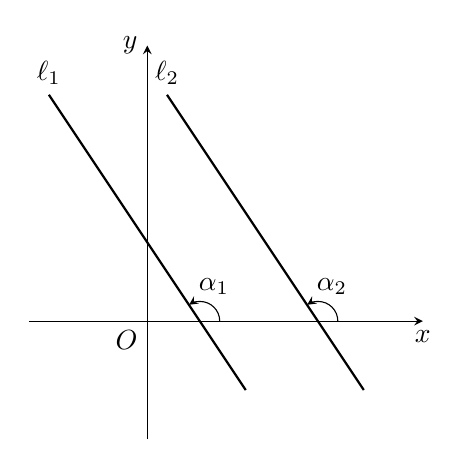
\begin{tikzpicture}[>=stealth]
    \draw[->](-1.5,0)--(3.5,0)node[below]{$x$};
    \draw[->](0,-1.5)--(0,3.5)node[left]{$y$};
    \node[below left]{$O$};
    \draw[domain=1.25:-1.25, thick, smooth]plot(\x, -1.5*\x+1)node[above]{$\ell_1$};
    \draw[domain=1.25:-1.25, thick, smooth]plot(\x+1.5, -1.5*\x+1)node[above]{$\ell_2$};.
    \draw[->](0.67+.25,0)arc (0:123.7:.25)node[above right]{$\alpha_1$};
    \draw[->](0.67+1.75,0)arc (0:123.7:.25)node[above right]{$\alpha_2$};
\end{tikzpicture}
\captionof{figure}{}
\end{minipage}

\begin{equation}
    \ell_1\parallel \ell_2 \text{（或$\ell_1$ 与$\ell_2$重合）} \Longleftrightarrow k_1=k_2  \tag{1}
\end{equation}

对于(1)要注意它的前提是$\ell_1,\ell_2$都存在斜率.


\subsection{垂直条件}
当$\ell_1\bot\ell_2$时，到角$\theta_{1-2}=\frac{\pi}{2}$，$\tan\theta_{1-2}$不存在，我们把到角公式写成
\begin{equation}
    \cot \theta_{1-2}=\frac{1+k_2k_1}{k_2-k_1} \tag{*}
\end{equation}


若$\ell_2\bot \ell_2$, 到角$\theta_{1-2}=\frac{\pi}{2}\quad \Rightarrow\quad \cot\theta_{1-2}=0$
\[\begin{cases}
    1+k_2k_1=0\\
    k_2-k_1\ne 0
\end{cases}\Rightarrow\quad k_1k_2=-1\]

若$k_1k_2=-1$
\[\begin{cases}
    1+k_2k_1=0\\
    k_2-k_1\ne 0
\end{cases}\Rightarrow\quad \cot\theta_{1-2}=0\quad \Rightarrow\quad    \theta_{1-2}=\frac{\pi}{2}\quad \Rightarrow\quad \ell_1\bot\ell_2\]

$\therefore\quad \ell_1\bot\ell_2 \Longleftrightarrow k_1k_2=-1$ \hfill(2)

注意：(2)成立的前提也是$\ell_1,\ell_2$都存在斜率.

(1)与(2)也可用$\ell_1,\ell_2$的方程的系数表示：

设$\ell_1:\; a_1x+b_1y+c_1=0$, $\ell_2:\; a_2x+b_2y+c_2=0$.

把$k_1=-\frac{a_1}{b_2}$, $k_2=-\frac{a_2}{b_2}$代入(1)，得
\begin{equation}
    k_1=k_2\Longleftrightarrow a_1b_2-a_2b_1=0\quad \text{（平行或重合）} \tag{3}
\end{equation}
代入(2)，得
\begin{align}
    k_1k_2=-1 &\Longleftrightarrow \left(-\frac{a_1}{b_1}\right)\left(-\frac{a_2}{b_2}\right)=-1 \nonumber\\
    &\Longleftrightarrow a_1a_2+b_1b_2=0 \quad \text{（垂直）} \tag{4}
\end{align} 

经验证，知道：
\begin{thm}{结论1}
    若$\ell_1$或$\ell_2$的斜率不存在，(3)和(4)仍然成立. 即：
\[\begin{split}
    \ell_1\parallel \ell_2 \text{（或$\ell_1$与$\ell_2$重合）} &\Longleftrightarrow a_1b_2-a_2b_1=0\\
    \ell_1\bot \ell_2  &\Longleftrightarrow a_1a_2+b_1b_2=0\\
\end{split}\]
\end{thm}


\begin{thm}{结论2}
    若$\ell$的方程是$ax+by+c=0$,
\begin{enumerate}[(1)]
\item 与$\ell$平行的直线的一般形式是：
\begin{equation}
    ax+by+m=0\quad \text{（$m$是参数）} \tag{5}
\end{equation}

\item 与$\ell$垂直的直线的一般形式是：
\begin{equation}
    bx-ay+m=0\quad \text{（$m$是参数）} \tag{6}
\end{equation}
\end{enumerate}
\end{thm}

这两条结论在应用上很重要，证明留给读者.





\begin{example}
已知直线$\ell_1:\; 2x-4y+7=0$，$\ell_2:\; x-2y+5=0$，
    求证：$\ell_1\parallel \ell_2$
\end{example}

\begin{analyze}
    只要证出$k_1=k_2$且其纵截距不相等即可.
\end{analyze}

\begin{solution}
    把$\ell_1,\ell_2$的方程写成斜截式：
\[\ell_1:\; y=\frac{1}{2}x+\frac{7}{4},\qquad \ell_2:\; y=\frac{1}{2}x+\frac{5}{2}\]
则$\ell_1$的斜率$k_1=\frac12$, 纵截距$b_1=\frac74$； $\ell_2$的斜率$k_2=\frac12$, 纵截距$b_2=\frac52$

$\therefore\quad k_1=k_2,\; b_1\ne b_2\quad \Rightarrow\quad \ell_1\parallel \ell_2$
\end{solution}


\begin{example}
    求过点$(2,1)$且与直线$\ell_1:\; 2x+y-10=0$垂直的直线$\ell_2$的方程.
\end{example}

\begin{analyze}
    利用$\ell_1\bot\ell_2\Longleftrightarrow k_1k_2=-1$可求得$\ell_2$的斜率$k_2$，再用点斜式可写出$\ell_2$ 的方程. 也可用本节结论(6)去作.
\end{analyze}

\begin{solution}
\textbf{解法1：}容易得出，$\ell_1$的斜率$k_1=-2$，由$\ell_1\bot\ell_2\Longleftrightarrow k_1k_2=-1$，可得
\[(-2)\cdot k_2=-1\Longleftrightarrow k_2=\frac{1}{2}\]
又因$\ell_2$过$(2,1)$点，知其方程是
\[y-1=\frac{1}{2}(x-2)\quad \Rightarrow\quad x-2y=0\]

\textbf{解法2：}由$\ell_1\bot \ell_2$，且$\ell_1$的方程是$2x+y-10=0$，知$\ell_2$的方程应具有形式
\begin{equation}
    x-2y+m=0  \tag{*}
\end{equation}

又$\because\quad \ell_2$过点$(2,1)$，

$\therefore\quad $点$(2,1)$的坐标应适合(*)，即
\[2-2\x1+m=0\quad \Rightarrow\quad m=0\]

$\therefore\quad \ell_2$的方程是$x-2y=0$.
\end{solution}

\begin{example}
    用坐标法解：
正方形$ABCD$中，$E$是$BC$边的中点，$F$是$AB$延长线上的一点，问$F$在什么位置时，$AE\bot CF$成立？
\end{example}

\begin{analyze}
如图2.14建立坐标系，设$F(x,0)$，利用$AE\bot CF\Longleftrightarrow k_{AE}\cdot k_{CF}=-1$，建立以$x$为“元”的方程，求$x$即可.
\end{analyze}

\begin{solution}
如图2.14建立坐标系，则有$B(1,0)$、$C(1,1)$、$D(0,1)$、$E\left(1,\frac{1}{2}\right)$. 设$F$的坐标为$(x,0)$. 显然，直线$AE$、$CF$的斜率都存在：
\[  k_{AE}=\frac{\frac{1}{2}-0}{1-0}=\frac{1}{2},\quad
    k_{CF}=\frac{1-0}{1-x}=\frac{1}{1-x}
 \]
利用$AE\bot CF\Longleftrightarrow k_{AE}\cdot k_{CF}=-1$，得
\[\frac{1}{2}\cdot \frac{1}{1-x}=-1\quad \Rightarrow\quad x=\frac{3}{2}\]
$\therefore\quad $当$BF=\frac{1}{2}AB$时就有$AE\bot CF$.
\end{solution}


\noindent
\begin{minipage}{.45\textwidth}
\centering
\begin{tikzpicture}[>=stealth]
\draw[->](-1,0)--(4,0)node[below]{$x$};
\draw[->](0,-1)--(0,4)node[left]{$y$};
\node[below left]{$A(O)$};
\tkzDefPoints{0/2/D, 3/0/F, 2/0/B, 2/2/C, 2/1/E,0/0/A}
\draw(D)--(C)--(B);
\draw(F)--(C);
\node at (B)[below, text width=1cm, align=center]{$B$\\$(1,0)$};
\node at (F)[below, text width=1cm, align=center]{$F$\\$(x,0)$};
\node at (C)[right]{$C(1,1)$};
\node at (D)[above right]{$D(0,1)$};
\tkzInterLL(A,E)(C,F) \tkzGetPoint{G}
\draw(A)--(G);
\node at (E)[left]{$E$};
\tkzMarkRightAngle[size=.2](A,G,F);
\end{tikzpicture}
\captionof{figure}{}
\end{minipage}
\hfill
\begin{minipage}{.45\textwidth}
\centering
\begin{tikzpicture}[>=stealth, scale=.5]
\tkzDefPoints{3/-4/A, 1/3/B, -4/-2/C}
\tkzDrawPolygon(A,B,C)
\tkzLabelPoints[left](C)
\tkzLabelPoints[above](B)
\node at (A)[right]{$A(3,-4)$};
\tkzDefPointBy[projection=onto B--A](C) \tkzGetPoint{E}
\tkzDefPointBy[projection=onto C--A](B) \tkzGetPoint{F}
\tkzDrawLines[add=0 and .3](C,E B,F)
\tkzMarkRightAngles[size=.3](C,E,A B,F,A)
\node at (3.5,0.5){$\ell_2$};
\node at (-1.5,-5){$\ell_1$};

\end{tikzpicture}
\captionof{figure}{}
\end{minipage}


\begin{example}
在$\triangle ABC$中，已知$A(3,-4)$和分别过点$B$、$C$的两条高所在的直线方程是$\ell_1:\; 7x-2y-1=0$与$\ell_2:\; 2x-7y-6=0$，求三边所在的直线的方程.
\end{example}

\begin{analyze}
    做解析几何题，画出图，直观形象，便于数形结合.但是，有时画图不易（如这里要在坐标系中画出$\triangle ABC$就不容易）.这时，可以画示意图代替在坐标系中画图.
\end{analyze}

\begin{solution}
    画出示意图（图2.15).

$\because\quad $直线$AC\bot \ell_1$, $\ell_1$的方程是：$7x-2y-1=0$,

$\therefore\quad AC$的方程具有形式$2x+7y+m=0$.

又$\because\quad AC$过$A(3,-4)$，可定出$m=22$,

$\therefore\quad AC$的方程是$2x+7y+22=0$

同理，$AB$的方程可求出，为$7x+2y-13=0$. 

点$B(x,y)$可由$\begin{cases}
    7x-2y-1=0\\ 7x+2y-13=0
\end{cases}$求出，为$B(1,3)$；

点$C(x,y)$可由$\begin{cases}
    2x-7y-6=0\\ 2x+7y+22=0
\end{cases}$求出，为$C(-4,-2)$.

$\therefore\quad BC$的方程是$y-3=\frac{3-(-2)}{1-(-4)}(x-1)$，即
\[x-y+2=0\]
\end{solution}

\begin{ex}
\begin{enumerate}
    \item 判断下列各对直线是否平行、垂直或重合：
\begin{enumerate}[(1)]
\item $y=3x+4$ 与 $2y-6x+1=0$;
\item $y=x$ 与 $3x+3y-10=0$;
\item $3x+4y-5=0$ 与 $6x-8y-7=0$;
\item $\sqrt{3}x-y-1=0$ 与 $\sqrt{3}x+3y+6=0$;
\item $\sqrt{2}x+\sqrt{3}y=\sqrt{6}$ 与 $2x+\sqrt{6}y-2\sqrt{3}=0$.
\end{enumerate}

    \item 求过点$A(2,3)$，且分别适合下列条件的直线方程：
\begin{enumerate}[(1)]
    \item 平行于直线$2x+y-7=0$;
    \item 垂直于直线$3x-2y+5=0$.
\end{enumerate}
    \item 已知两直线$\ell_1,\ell_2$，其中$\ell_1$没有斜率. $\ell_1$与$\ell_2$什么时候
    （1）平行；（2）垂直？其逆命题成立吗？
\end{enumerate}
\end{ex}

\section{两条直线的交点}
设两条直线为
\[\begin{split}
 \ell_1:&\; a_1x+b_1y+c_1=0\\
\ell_2:&\; a_2x+b_2y+c_2=0   
\end{split}\]

根据1.4节的推论，求$\ell_1$、$\ell_2$的交点的问题等价于解方程组
\[\begin{cases}
    a_1x+b_1y+c_1=0 &(1)\\
    a_2x+b_2y+c_2=0 &(2)
\end{cases}\]
的问题.

\begin{itemize}
    \item 若方程组有唯一解$(x_0,y_0)$，则$\ell_1$、$\ell_2$相交于$(x_0,y_0)$;
    \item 若方程组无解，则$\ell_1\parallel \ell_2$；
    \item 若方程组有无穷多解，则$\ell_1$重合于$\ell_2$．
\end{itemize}

设$a_1$、$a_2$、$b_1$、$b_2$全不为零，解这个方程组：

$(1)\times b_2$，得
\begin{equation}
    a_1b_2x+b_1b_2y+b_2c_1=0 \tag{3}
\end{equation}
$(2)\times b_1$，得
\begin{equation}
    a_2b_1x+b_1b_2y+b_1c_2=0 \tag{4}
\end{equation}
$(3)-(4)$得
\[(a_1b_2-a_2b_1)x+(b_2c_1-b_1c_2)=0\]
即
\begin{equation}
    (a_1b_2-a_2b_1)x=b_1c_2-b_2c_1 \tag{5}
\end{equation}

\begin{enumerate}
    \item 当$a_1b_2-a_2b_1\neq0$时，(5)有唯一解，从而可求出方程
组的唯一解：
\[\begin{cases}
    x=\frac{b_1c_2-b_2c_1}{a_1b_2-a_2b_1}\\
    y=\frac{a_2c_1-a_1c_2}{a_1b_2-a_2b_1}
\end{cases}\]
这时，$\ell_1,\ell_2$相交，上面$x$和$y$ 的值就是交点的坐标. 这是因为$\ell_1,\ell_2$的斜率分别是$-\frac {a_1}{b_1}$和$-\frac{a_2}{b_2}$, 由$a_1b_2-a_2b_1\neq0$可知$\frac{a_1}{b_1}\neq\frac{a_2}{b_2}$, 也就是$-\frac {a_1}{b_1}\neq-\frac{a_2}{b_2}$, 这说明$\ell_1,\ell_2$的斜率不等，所以$\ell_1,\ell_2$必相交于一点.

例如，两条直线
\[\begin{split}
    2x-3y+4&=0\\
    3x+y-5&=0
\end{split}\]
由于$\frac23\neq\frac3{-1}$（斜率不等），也就是$\frac23\neq\frac{-3}1$（$x$、$y$项的对应
系数不成比例），这两个方程组成的方程组就有唯一解，这个
解是
$$\begin{cases}x=1\\y=2\end{cases}$$
也就是两条直线相交于点$(1,2)$.

\item 当$a_1b_2-a_2b_1=0$时，
\begin{enumerate}[(i)]
    \item  若 $b_1c_2-b_2c_1\neq0$，(5)无解，从而方程组无解. 事实上，这时$c_1,c_2$不可能全为零，不妨设$c_2\neq0$, 有$\frac {a_1}{a_2}=\frac{b_1}{b_2}\neq\frac{c_1}{c_2}$, 也就是$\frac{a_1}{b_1}=\frac{a_2}{b_2}$, 且$\frac {c_1}{b_1}\neq\frac{c_2}{b_2}$, 所以，$\ell_1,\ell_2$的斜率相等：$-\frac{a_1}{b_1}=-\frac{a_2}{b_2}$, 
而纵截距不等，$\frac{c_1}{b_1}\neq\frac{c_2}{b_2}$, 此时，$\ell_1\parallel \ell_2$.

例如，两条直线
\[\begin{split}
    3x-y+2&=0\\6x-2y-5&=0
\end{split}\]
由于$\frac{3}{6}=\frac{-1}{-2}\ne\frac{2}{-5}$，所以方程组无解，也就是两直线平行.
\item 若$b_1c_2-b_2c_1=0$，(5)有无穷多解，从而方程组也有无穷多解. 事实上，此时$c_1$、$c_2$ 或全为零或全不为零（当$c_1,c_2$ 全不为零时，$\frac{a_1}{a_2}=\frac{b_1}{b_2}=\frac{c_1}{c_2}$），两个方程是同解方程，所以它们有无穷多解，也就是两条直线重合.

例如，两条直线
\[\begin{split}
    3x-y+2&=0\\
    6x-2y+4&=0
\end{split}\]
由于$\frac{3}{6}=\frac{-1}{-2}=\frac{2}{4}$, 两个方程是同解方程，方程组有无穷多
解，因而两直线重合.
\end{enumerate}
\end{enumerate}

对于$a_1,a_2,b_1,b_2$有等于零的情况，方程组比较简单，
同学们可自己进行讨论.








\begin{example}
    根据下列每组直线的方程判断两条直线的位置关系（相交？平行？重合？），若相交，求出交点坐标：
\begin{enumerate}[(1)]
\item $\ell_1:\; 3x-2y-6=0;\qquad \ell_2:\; 9x+4y+7=0$
\item $\ell_1:\; 3x-2y-6=0;\qquad \ell_2:\; 4y-6x-3=0$
\end{enumerate}
\end{example}
 
\begin{solution}
\begin{enumerate}[(1)]
    \item 解方程组$\begin{cases}
        3x-2y=6\\ 9x+4y=-7
    \end{cases}$
得
$\begin{cases}
    x=\frac{1}{3}\\y=-\frac{5}{2}
\end{cases}$

$\ell_1,\ell_2$相交于$\left(\frac{1}{3},-\frac{5}{2}\right)$
\item 解方程组
$\begin{cases}
    3x-2y=6\\ -6x+4y=3
\end{cases}$

$\because\quad \frac{3}{-6}=\frac{-2}{4}\ne \frac{6}{3}$

$\therefore\quad \ell_1,\ell_2$平行.
\end{enumerate}
\end{solution}


\begin{example}
    已知两直线
\[\begin{split}
  \ell_1:&\; x+my+6=0\\
  \ell_2:&\; (m-2)x+3y+2m=0 
\end{split}\]
求当$m$为何值时，$\ell_1$与$\ell_2$：（i）相交；（ii）平行；（iii）重合.
\end{example}

\begin{solution}
解方程组$\begin{cases}
    x+my=-6\\ (m-2)x+3y=-2m
\end{cases}$
\[\begin{split}
  a_1b_2-a_2b_1&=1\x3-(m-2)m=3-m^2+2m\\
b_1c_2-b_2c_1&=m(-2m)-3(-6)=-2m^2+18  
\end{split}\]

令$a_1b_2-a_2b_1=0$，即$-m^2+2m+3=0$，解得$m=3$, $m=-1$.

令$b_1c_2-b_2c_1=0$，即$-2m^2+18=0$，解得$m=\pm 3$.

\begin{enumerate}[(i)]
\item 当$m\ne 3$，且$m\ne -1$时，$a_1b_2-a_2b_1\ne 0$，方程组有唯一解，$\ell_1$与$\ell_2$相交；
\item 当$m=-1$时，$a_1b_2-a_2b_1=0$, $b_1c_2-b_2c_1\ne 0$，方程组无解，$\ell_1$与$\ell_2$平行；
\item 当$m=3$时，$a_1b_2-a_2b_1=0$，$b_1c_2-b_2c_1=0$，方程组有无穷多解，$\ell_1$与$\ell_2$重合． 
\end{enumerate}
\end{solution}

\begin{ex}
\begin{enumerate}
    \item 求下列各对直线的交点，并画图：
\begin{enumerate}[(1)]
    \item $\ell_1:\; 2x-y=1,\qquad \ell_2:\; 3x+2y=19$
    \item $\ell_1:\; x=2,\qquad \ell_2:\; 3x+2y-12=0$
\end{enumerate}

    \item 判定下列各对直线的位置关系.若相交，求出交点坐标：
\begin{enumerate}[(1)]
\item $4x-3y-8=0$与$3x-y=0$;
\item $2x-6y+4=0$与$y=\frac{x}{3}+\frac{2}{3}$;
\item $(\sqrt{2}-1)x+y=3$与$x+(\sqrt{2}+1)y=2$;
\item $2x-3y=5$与$4x-6y=10$.
\end{enumerate}

    \item 当$a$，$b$取何值时，直线$ax-2y-1=0$与$6x-4y-b=0$.
\begin{multicols}{3}
\begin{enumerate}[(1)]
    \item 相交；
    \item 平行；
    \item 重合．
\end{enumerate}
\end{multicols}
    \item 已知直线满足下列条件，求直线的方程：
\begin{enumerate}[(1)]
\item 过直线$3x-y+4=0$与$x+y-4=0$的交点，且斜率为$-2$；
\item 过直线$x-2y+3=0$与$x+2y-9=0$的交点和原点.
\end{enumerate}

\end{enumerate}
\end{ex}

\section*{习题二}
\begin{center}
    \bfseries A
\end{center}

\begin{enumerate}
    \item  已知直线$\ell:\; y=x+5$. 求过点$A(5,2)$且与直线$\ell$的夹角为$45^{\circ}$的直线的方程．
    \item 已知三角形三边所在的直线方程分别是：
\[\begin{split}
    AB:&\; x-y-3=0\\
    BC:&\; x-3y+3=0\\
    AC:&\; 2x+y+5=0\\
\end{split}\]
    试求三个内角（用反三角函数表示）.
    \item 已知两点$A(2,2)$、$B(5,-2)$．在横轴上求一点$P$，使$\angle APB$为直角．你还能把此题推广吗？
    \item 直线$(3a+2)x+(1-4a)y+8=0$和$(5a-2)x+(a+4)y-7=0$互相垂直. 试求$a$的值. 提示：利用本节结论(4).
    \item 求证：对于$\alpha\in [0,\pi]$，直线
    $x\sin\alpha+y\cos\alpha+1=0$
    总与直线
    $x\cos\alpha-y\sin\alpha+2=0$
    垂直.
    \item 求证：直线$x+2y-5=0$, $2x+4y+5=0$, $2x-y=0$, $7x-11y-35=0$围成一个直角梯形.
    \item 直线$ax+2y+8=0$, $4x+3y=10$和$2x-y=10$相交于一点，求$a$值.
    \item 不解方程组，判断下列两方程的直线的位置关系：
\begin{multicols}{2}
\begin{enumerate}[(1)]
    \item $\begin{cases}
        3x-y=4\\ 2x+3y=5
    \end{cases} $
    \item $\begin{cases}
        3x+2y=6\\ 6x+4y=12
    \end{cases} $
    \item $\begin{cases}
        x-3y=-4\\3x-9y=10
    \end{cases} $
    \item $\begin{cases}
        12x-6y=-6 \\ 8x-4y=4
    \end{cases} $
\end{enumerate}
\end{multicols}
\end{enumerate}

\begin{center}
    \bfseries B
\end{center}

\begin{enumerate}\setcounter{enumi}{8}
    \item  直线上依次有四个点$A$、$B$、$C$、$D$，且$AB=BC=CD$. $P$为以$BC$为直径的半圈上的任一点（$P$与$B$、$C$都不重合）. 记$\angle APB=\alpha$, $\angle CPD=\beta$，求证$\tan\alpha\cdot \tan\beta$为定值.
    \item 已知两条直线
\[\begin{split}
     \ell_1:&\; (3+m)x+4y=5-3m\\
    \ell_2:&\; 2x+(5+m)y=8   
\end{split}\]
$m$为何值时，$\ell_1$
    与$\ell_2$：
    （1）相交；（2）平行；（3）重合．
    \item 若$P(a,b)$为第一象限内的一个定点，过点$P$的动直线交$x$、$y$轴的正方向于$M$、$N$. 求证：$\triangle OMN$面积的最小值为$2ab$．
\end{enumerate}

\section*{三、点与直线的位置关系}
点与直线的位置关系可分为两类：一是点在直线上，一是点不在直线上. 对于已知点$A$的坐标，和直线$\ell$的方程时，如何判断点$A$在直线$\ell$上或不在$\ell$上我们已讨论过了. 下面讨论当$A$不在直线$\ell$上时，如何求$A$到直线$\ell$的距离. 以及点$A$关于直线$\ell$的对称点的坐标的求法.











\begin{example}
    
\end{example}

\begin{analyze}
    
\end{analyze}

\begin{solution}
    
\end{solution}






\begin{example}
    
\end{example}

\begin{analyze}
    
\end{analyze}

\begin{solution}
    
\end{solution}


\begin{example}
    
\end{example}

\begin{analyze}
    
\end{analyze}

\begin{solution}
    
\end{solution}



\begin{example}
    
\end{example}

\begin{analyze}
    
\end{analyze}

\begin{solution}
    
\end{solution}


































































































































































